% !TEX program = xelatex
\documentclass[10pt,letterpaper,twocolumn]{article}

% === PAGE ===
\usepackage[top=0.75in,bottom=0.75in,left=0.75in,right=0.75in,footskip=12pt]{geometry}

% === FONTS ===
\usepackage{fontspec}
\usepackage{unicode-math}
\setmainfont{Latin Modern Roman}[
  Extension=.otf,
  UprightFont=lmroman10-regular,
  BoldFont=lmroman10-bold,
  ItalicFont=lmroman10-italic,
  BoldItalicFont=lmroman10-bolditalic,
]
\setsansfont{Latin Modern Sans}[
  Extension=.otf,
  UprightFont=lmsans10-regular,
  BoldFont=lmsans10-bold,
  ItalicFont=lmsans10-oblique,
  BoldItalicFont=lmsans10-boldoblique,
]
\setmonofont{Latin Modern Mono}[
  Extension=.otf,
  UprightFont=lmmono10-regular,
  ItalicFont=lmmono10-italic,
  Scale=0.85,
]
\newfontfamily\acbold{ywft-processing-bold}[
  Path=../../system/public/type/webfonts/,
  Extension=.ttf
]

% === PACKAGES ===
\usepackage{xcolor}
\usepackage{titlesec}
\usepackage{enumitem}
\usepackage{booktabs}
\usepackage{tabularx}
\usepackage{array}
\newcolumntype{Y}{>{\RaggedRight\arraybackslash}X}
\newcolumntype{R}[1]{>{\RaggedRight\arraybackslash}p{#1}}
\usepackage{fancyhdr}
\usepackage{hyperref}
\usepackage{xurl}
\usepackage{graphicx}
\graphicspath{{./}{figures/}}
\usepackage{ragged2e}
\usepackage{microtype}
\usepackage[font=footnotesize]{caption}
\usepackage{natbib}
\usepackage{tikz}
\usetikzlibrary{arrows.meta,calc,positioning}
\usepackage{../ac-source-bundle}

% === COLORS ===
\definecolor{acpink}{RGB}{180,72,135}
\definecolor{acpurple}{RGB}{120,80,180}
\definecolor{acdark}{RGB}{64,56,74}
\definecolor{acgray}{RGB}{119,119,119}

\hypersetup{
  colorlinks=true,
  linkcolor=acpurple,
  urlcolor=acpurple,
  citecolor=acpurple,
  pdfauthor={@jeffrey},
  pdftitle={Don't Forget the Keyboard: Laptop Performance, Typed Music, and Where notepat Stands},
}

% === SECTIONS ===
\titleformat{\section}{\normalfont\bfseries\normalsize\uppercase}{\thesection.}{0.5em}{}
\titlespacing{\section}{0pt}{1.2em}{0.3em}
\titleformat{\subsection}{\normalfont\bfseries\small}{\thesubsection}{0.5em}{}
\titlespacing{\subsection}{0pt}{0.8em}{0.2em}

% === RUNNING MATTER ===
\pagestyle{fancy}
\fancyhf{}
\renewcommand{\headrulewidth}{0pt}
\fancyfoot[C]{\footnotesize\thepage}
\setlist[itemize]{nosep,leftmargin=1.2em,itemsep=0.1em}
\setlist[enumerate]{nosep,leftmargin=1.4em,itemsep=0.1em}
\setlength{\columnsep}{1.8em}
\setlength{\parindent}{1em}
\setlength{\parskip}{0.3em}
\tolerance=800
\emergencystretch=2em
\hyphenpenalty=50

\newcommand{\acdot}{{\color{acpink}.}}
\newcommand{\ac}{Aesthetic{\acdot}Computer}
\newcommand{\acos}{AC Native OS}
\newcommand{\np}{\texttt{notepat}}
\newcommand{\code}[1]{\texttt{#1}}
\newcommand{\key}[1]{\texttt{#1}}
\newcommand{\term}[1]{``#1''}

\InputIfFileExists{version}{}{%
  \providecommand{\paperhash}{dev}\providecommand{\paperrev}{?}}

\begin{document}

\twocolumn[{%
\begin{center}
{\acbold\fontsize{24pt}{28pt}\selectfont\color{acdark} Don't Forget the Keyboard}\par
\vspace{0.45em}
{\itshape\fontsize{13.5pt}{16.5pt}\selectfont\color{acpink} Laptop Performance, Typed Music, and Where \np{} and \acos{} Stand}\par
\vspace{0.6em}
{\small\color{acgray} \href{https://prompt.ac/@jeffrey}{@jeffrey} \,\textperiodcentered\, \ac{} \,\textperiodcentered\, ORCID \href{https://orcid.org/0009-0007-4460-4913}{0009-0007-4460-4913} \,\textperiodcentered\, November 2026}\par
\vspace{0.55em}
{\color{acpink}\rule{\textwidth}{1.2pt}}
\vspace{0.5em}
\end{center}

\begin{quote}
\small\noindent\textbf{Abstract.}
The laptop has been a performed instrument for twenty years, and its keyboard has been a note-entry device for forty. This paper maps that field and places two \ac{} systems in it: \np{}, a chromatic instrument whose letter keys play the notes they name, and \acos{}, which boots a surplus laptop straight into \np{}. From 68 sources gathered in one search pass and indexed in a new \texttt{laptop-platter}, I trace eight threads: typewriter percussion, tracker note entry, typed-letter notation communities, laptop orchestras and the native-input program, named key-mapping logics, typing as the musical gesture, the liveness critique, and computers booted into instruments. Then I test four claims about where \ac{} stands. Two survive narrowly. I found no earlier instrument that maps letters to their own note names, and no earlier system that boots an ordinary laptop into one instrument played on its own keys. dyne:bolic, Puredyne and MOD's live USB come close, and they set the boundary. One claim is measured: key-to-sound latency of 3--4\,ms on HDA hardware, inside Wessel and Wright's 10\,ms budget. One claim, that a typed melody answers the critique that a laptop player could be checking email, is argued but untested. For each claim I name the study that would settle it.
\end{quote}
\vspace{0.5em}
}]

\section{The Question}

Someone asked whether anyone else had done this: played melodies on a computer keyboard, or mashed out beats on one, the way \np{} does. The honest answer is yes, a lot of people, for a long time. The useful answer is a map. Who did it, how they mapped the keys, what hardware they ran on, what critics said about it, and which parts of \np{} and \acos{} fall in empty space on that map.

This paper is that map. It sits beside three earlier \ac{} papers that already hold part of the ground. \emph{Keymaps as Social Software} traces the keymap lineage from Sholes to Wicki--Hayden, names the DAW's QWERTY-piano convention the \emph{AWSED} layout, and argues for \np{}'s ``notes that name themselves''~\citep{scudder2026keymaps}. \emph{PLORKing the Planet} covers laptop orchestras~\citep{scudder2026plork}. \emph{Where the Microseconds Go} walks the key-to-DAC path~\citep{scudder2026latency}. Here I widen the frame to the whole genre of laptop performance and ask a narrower question: where exactly is the boundary of what \ac{} has that the field does not?

\section{Sources and Method}

I searched the public web through \ac{}'s own search service, which is backed by Exa and keeps no query logs. 30 queries ran on 2 November 2026: research on QWERTY melodic input, tapped rhythm entry, laptop orchestras, typing-to-music toys, isomorphic layouts, rollover and latency, the liveness critique, dedicated music operating systems and live distributions, tracker history, typed-letter notation communities, and the theory of instrument constraint. For each candidate I retrieved the primary page (a proceedings PDF, a publisher table of contents, a project page) and read the citation off it. Where I wrote an author or page from memory, I checked it. One author list I had wrong (the 2019 Taptop paper) was corrected from the PDF.

The result is a new sub-platter, \texttt{papers/laptop-platter/}: 68 sources on ten shelves, 66 checked against a primary page, with a query log and a table of \emph{negative searches}, meaning the claims of absence and the queries behind them. Products, web toys and community sites are cited as evidence that a practice exists, never as authority on whether it works.

\section{Typing Was Percussion First}

The keyboard was a drum before it was a controller. Leroy Anderson's \emph{The Typewriter} (completed 1950, recorded 1953) treats a manual typewriter as a solo percussion part. The machine was modified so only two keys worked, and Anderson said only drummers had the wrist speed to play it~\citep{anderson1950typewriter}. The Boston Typewriter Orchestra, founded in 2004, still plays desk machines from the 1910s for their shift-key thump. Its members report the same ceiling: when they try to tap out a melody, no one can tell what they are playing~\citep{bto2004}.

That ceiling is the starting condition for everything below. A key gives you an onset and nothing else. Pitch has to come from a mapping.

\section{The Keyboard as a Note-Entry Device}

The mapping most people meet first came from game music. Chris H\"ulsbeck's Soundmonitor (Commodore~64, 1986) wrote music as text: a letter, an optional sharp, an octave digit~\citep{borderie2023soundmonitor}. Karsten Obarski's Ultimate Soundtracker (Amiga, 1987) added the move that stuck. Two rows of letter keys act as the white keys of a piano, and the row above each acts as the black keys. Nearly every tracker since has kept it~\citep{cant2020trackers}. Scream Tracker's 1990 manual lays the two octaves on the \key{Z} and \key{Q} rows. It also adds a separate shifted ``beat keyboard'' for entering drums, an early sign that pitch entry and beat entry want different layouts~\citep{screamtracker1990}.

GarageBand's Musical Typing moved the octave to the home row, with \key{Z}/\key{X} for octave and \key{C}/\key{V} for velocity~\citep{owen2018musicaltyping}. Ableton, Logic and FL Studio ship variants of the same layout, and so does every web piano I found. That is the convention \emph{Keymaps} names AWSED, after the keys of its first five chromatic tones~\citep{scudder2026keymaps}. Its defining property is that the key's letter has nothing to do with the note: \key{A} plays C.

\paragraph{The vernacular branch.} A very large community already writes music as typed letters and has not been studied. Virtual Piano and the Roblox piano games use \emph{sheets}: songs written as the characters to press, with lowercase for white keys, uppercase for black keys, brackets for chords and dashes for rests~\citep{virtualpiano_sheets}. One aggregator listed 51{,}613 sheets on the day I checked~\citep{pianoglow_sheets}. This is a living notation, transmitted by copy and paste, mostly by young players. The letters in it name keys, not pitches. A sheet for one site's layout is gibberish on another. \np{}'s song encoding~\citep{scudder2026folksongs} is the same idea with the indirection removed, because in \np{} the letter is the pitch.

\section{The Laptop Orchestra and the Native-Input Program}

The academic genre begins at Princeton. PLOrk's first year (2005--06) put fifteen laptops with hemispherical speakers on stage~\citep{trueman2006plork}. Two of its first pieces played the keyboard itself. In Dan Trueman's \emph{ABC Song}, each player records their own voice saying the name of every key, and comb filters tune the spoken letters into the alphabet song, in three-part harmony with a conductor. In Ge Wang's \emph{CliX}, every key is mapped to a pitch by its ASCII code and clicks are quantized to a shared pulse~\citep{wang2006clix}. The ensemble's composers reported that ``the latency of the QWERTY keyboard [was] acceptable for most rhythmic playing''~\citep{smallwood2008composing}.

Fiebrink, Wang and Cook turned this into a program in \emph{Don't Forget the Laptop} (NIME 2007)~\citep{fiebrink2007laptop}. Their argument was practical. Custom controllers lengthen setup, break in transit, cost money and need maintenance, while every laptop already has a keyboard, a trackpad, a microphone and, in 2007, a motion sensor. They showed the keyboard as an ASCII pitch selector and as a fretboard, the trackpad as a bow, and the hard-drive motion sensor as a drum (\emph{Smacking Music}, Steve Reich's \emph{Clapping Music} played by hitting PowerBooks). They also shipped a toolkit, SMELT. The title of this paper is a nod to theirs.

The line continued: SLOrk at Stanford (2008), MoPhO for phones~\citep{wang2008mopho}, Laptap's microphone-to-speaker feedback played by touch~\citep{nime2013laptap}, and Taptop's trackpad grids~\citep{nime2019tops}. Wang's \emph{Artful Design} collects the philosophy~\citep{wang2018artful}. What the program never did was make the laptop \emph{only} an instrument. The orchestra laptop still ran a desktop, launched a ChucK or Max patch, and was configured by a technician before each concert. \emph{PLORKing the Planet} argues that this cost, not the music, kept laptop orchestras rare~\citep{scudder2026plork}.

\section{What a Key Means: Six Mapping Logics}

Every QWERTY instrument answers one question: given a key, which pitch? The answers I found fall into six families (Table~\ref{tab:mappings}).

\begin{table*}[t]
\centering
\footnotesize
\renewcommand{\arraystretch}{1.18}
\begin{tabularx}{\textwidth}{@{}R{2.25cm}R{3.7cm}YR{4.1cm}@{}}
\toprule
\textbf{Logic} & \textbf{Examples} & \textbf{What a key means} & \textbf{What the player must already know} \\
\midrule
Position & Ultimate Soundtracker 1987; Musical Typing; every web piano (AWSED) & Its place in two staggered rows imitates a white or black piano key. & The piano, and the layout itself. The letter tells you nothing. \\
Harmonic & aQWERTYon~\citep{hein2016inside} & Rows are scales, columns are diatonic chords; there are no wrong notes. & Nothing to start; theory to use the columns. In think-aloud tests no one found the column chords unprompted~\citep{hein2017welcoming}. \\
Isomorphic & Wicki--Hayden, Jank\'o on QWERTY~\citep{openmpt2016isomorphic,follington_qkeys} & Fixed interval per step in each direction, so every chord shape transposes. & The interval grid. \\
Code point & \emph{CliX}~\citep{wang2006clix} & ASCII value sets the pitch region. & Nothing. Melody is hard by design. \\
Frequency & \emph{TypistInstrument}~\citep{steiner2005typist}; US 6,444,888~\citep{patent6444888} & The most frequent letters (ETAOINSR) or the most-played notes get the scale. & Nothing. Typing English makes tonal music. \\
\textbf{Name} & \textbf{\np{}} (2024) & \textbf{The letter is the note: \key{c} plays C, \key{d} plays D; the next octave runs \key{h}--\key{n}.} & \textbf{The seven letter names of the Western scale.} \\
\bottomrule
\end{tabularx}
\caption{Six answers to ``which pitch does this key play?'' Five come from the literature and products surveyed here; the sixth is \np{}'s~\citep{scudder2026keymaps}. Only the last makes the printed letter on the key cap carry the pitch.}
\label{tab:mappings}
\end{table*}

The families are not ranked. Each one bets on a different piece of knowledge the player already has. AWSED bets on the piano and spends the keyboard to imitate it. aQWERTYon bets on nothing and prevents wrong notes, so its knowledge lives in the instrument, which is what Magnusson calls an \emph{epistemic tool}~\citep{magnusson2009epistemic}. Steiner's mapping bets on English: write a sentence and the letter statistics make it tonal. \np{} bets on literacy. Anyone who can spell \texttt{CDEFGAB} already knows where seven notes are.

Steiner is the nearest relative. His instrument also derives pitch from the letter rather than its position. But he chose frequency, not names: \key{e} and \key{t} become the tonic because they are common, not because they are E and T~\citep{steiner2005typist}.

\section{Typing as the Gesture}

\begin{figure*}[t]
\centering
% Positioning map: where the instrument lives (x) by what a key means (y).
% Cell contents are the systems surveyed in sections 3-8; sources in
% papers/laptop-platter/sources.json.
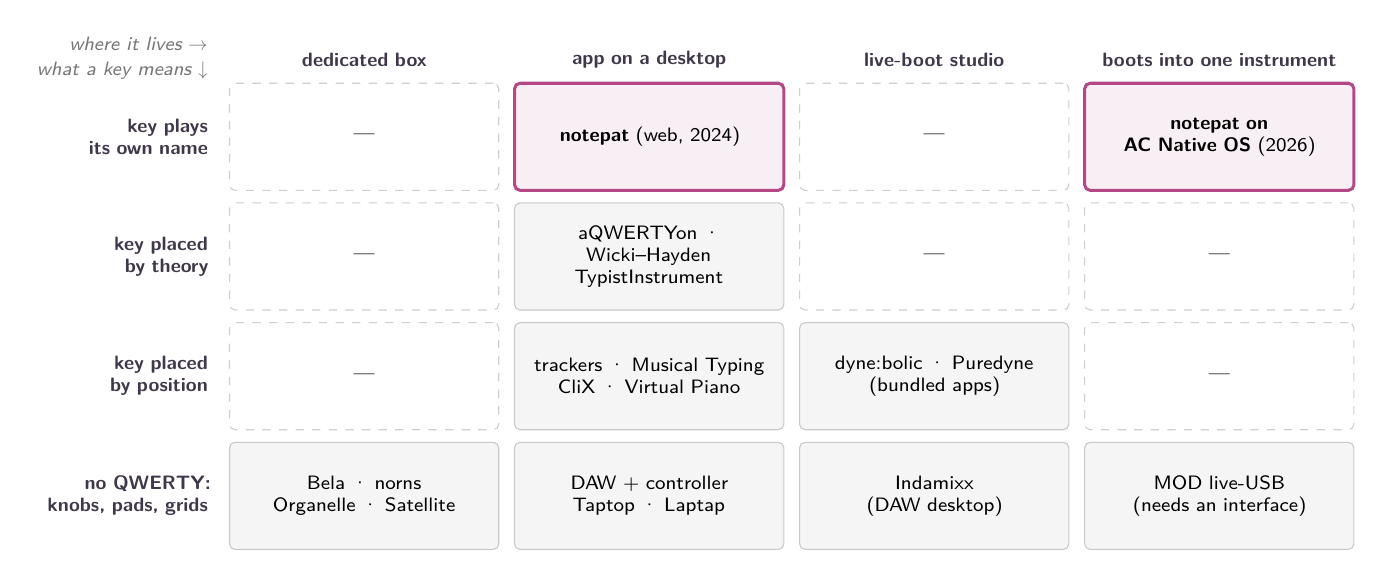
\begin{tikzpicture}[
  every node/.style={font=\sffamily},
  cell/.style={draw=acgray!40, fill=white, rounded corners=2pt,
    minimum width=3.42cm, minimum height=1.36cm, text width=3.1cm,
    align=center, font=\scriptsize\sffamily, inner sep=3pt},
  filled/.style={cell, fill=acgray!7},
  ours/.style={cell, draw=acpink, line width=1.1pt, fill=acpink!9},
  open/.style={cell, draw=acgray!35, dashed, fill=white, text=acgray},
  colhead/.style={font=\scriptsize\sffamily\bfseries, text=acdark, align=center, text width=3.3cm},
  rowhead/.style={font=\scriptsize\sffamily\bfseries, text=acdark, align=right, text width=2.15cm, anchor=east},
  axis/.style={font=\scriptsize\sffamily\itshape, text=acgray}
]
  \def\dx{3.62}\def\dy{1.52}
  % column x positions (cell centres)
  \def\cA{0}\def\cB{\dx}\def\cC{2*\dx}\def\cD{3*\dx}
  % row y positions, top row = by name
  \def\rN{0}\def\rT{-\dy}\def\rP{-2*\dy}\def\rC{-3*\dy}

  % column heads
  \node[colhead] at (\cA,0.98) {dedicated box};
  \node[colhead] at (\cB,0.98) {app on a desktop};
  \node[colhead] at (\cC,0.98) {live-boot studio};
  \node[colhead] at ({\cD},0.98) {boots into one instrument};

  % row heads
  \node[rowhead] at (-1.86,\rN) {key plays\\its own name};
  \node[rowhead] at (-1.86,\rT) {key placed\\by theory};
  \node[rowhead] at (-1.86,\rP) {key placed\\by position};
  \node[rowhead] at (-1.86,\rC) {no {QWERTY}:\\knobs, pads, grids};

  % row: by name
  \node[open]   at (\cA,\rN) {---};
  \node[ours]   at (\cB,\rN) {\textbf{notepat} (web, 2024)};
  \node[open]   at (\cC,\rN) {---};
  \node[ours]   at ({\cD},\rN) {\textbf{notepat on}\\\textbf{AC Native OS} (2026)};

  % row: by theory
  \node[open]   at (\cA,\rT) {---};
  \node[filled] at (\cB,\rT) {aQWERTYon \textperiodcentered\ Wicki--Hayden\\TypistInstrument};
  \node[open]   at (\cC,\rT) {---};
  \node[open]   at ({\cD},\rT) {---};

  % row: by position
  \node[open]   at (\cA,\rP) {---};
  \node[filled] at (\cB,\rP) {trackers \textperiodcentered\ Musical Typing\\CliX \textperiodcentered\ Virtual Piano};
  \node[filled] at (\cC,\rP) {dyne:bolic \textperiodcentered\ Puredyne\\(bundled apps)};
  \node[open]   at ({\cD},\rP) {---};

  % row: no qwerty
  \node[filled] at (\cA,\rC) {Bela \textperiodcentered\ norns\\Organelle \textperiodcentered\ Satellite};
  \node[filled] at (\cB,\rC) {DAW + controller\\Taptop \textperiodcentered\ Laptap};
  \node[filled] at (\cC,\rC) {Indamixx\\(DAW desktop)};
  \node[filled] at ({\cD},\rC) {MOD live-USB\\(needs an interface)};

  % axis captions, set in the empty corner above the row heads
  \node[axis, anchor=east, align=right] at (-1.86,1.0) {where it lives $\rightarrow$\\[1pt]what a key means $\downarrow$};
\end{tikzpicture}

\caption{The surveyed systems placed by where the instrument lives (columns) and what a key means (rows). Pink cells are \ac{}; dashed cells held nothing I found. dyne:bolic and Puredyne reach the third column through bundled applications with AWSED-style typing. MOD reaches the fourth without a QWERTY instrument. The top-right cell, a laptop booted into an instrument whose keys play their own names, is the boundary this paper defends. It is a claim about a search, not a proof of absence (§\ref{sec:limits}).}
\label{fig:positioning}
\end{figure*}

A second family treats the act of typing text as the music. Si Waite's NIME 2015 system drives melody, rhythm, timbre and projected visuals from typed lyrics, and argues that the visible link between keystroke and sound makes the performance feel live~\citep{waite2015keyboard}. Kyle Stetz's Typedrummer (2015) turns each letter into a drum hit, so a typed sentence is a beat~\citep{vanhemert2015typedrummer}. Orca (Hundred Rabbits, 2018) makes every letter of the alphabet a sequencer operator on a grid~\citep{orca2018}. The Stenophone points out that laptop live coding, whatever it sounds like, shares one physical interface, the QWERTY keyboard~\citep{stenophone2017}.

The newest entry is from this year's NIME. Encinas and Jensenius describe \emph{vyping}, typing to a language model without looking, as a musical practice in which typos act as grace notes and the model comps like a rhythm section~\citep{encinas2026vyping}. One of their artifacts is called \emph{clix-vibe}, after Wang's piece. They also name a gap: chat interfaces strip keystroke timing before it reaches the model, so the rhythm of typing is lost.

Beat mashing has its own small literature. Musipedia lets you search for a melody by tapping its rhythm on any key~\citep{typke_musipedia}. Claptoscore turns tapped rhythms into notation. It calibrates each input's latency separately, uses \key{F} and \key{J} as two percussion voices, and can read key release as note length~\citep{claptoscore}. An online study, \emph{tap the groove}, asks people to reduce full drum grooves to spacebar taps~\citep{tapthegroove}. Psychology adds one finding that matters here: the extra delay between same-hand keystrokes in typing does not appear in skilled piano playing~\citep{schmuckler1997interkey}. Typing skill and keyboard skill overlap without being the same skill.

\section{The Liveness Critique}

The genre's standing objection is visual. In 2003 \emph{Contemporary Music Review} gave a whole issue to the laptop as instrument, edited by Kim Cascone~\citep{cascone2003grain}. Cascone wrote that ``spectacle is the guarantor of presence and authenticity, whereas laptop performance represents artifice and absence.'' Caleb Stuart asked audiences to listen instead of watch~\citep{stuart2003object}. Nick Collins, in the same issue, put it most bluntly. A SuperCollider performer ``cannot be readily distinguished from someone checking their e-mail''~\citep{collins2003generative}.

Two answers followed. Live coders projected their screens~\citep{collins2003livecoding,mclean2010visualisation}. NIME built visible controllers and visualizations like Rouages, which reveal an instrument's mechanism to the audience~\citep{berthaut2013rouages}. Then Bown, Bell and Parkinson ran a listening test with audio only. Listeners heard \emph{triggering} as live, more than tweaking, and generative or prepared material did not cancel the effect~\citep{bown2014liveness}.

A typed melody is the extreme case of triggering. One key, one note, no automation in between, and on \np{} the note's letter is on the screen. That is an argument for why the critique should not apply. It has not been tested on \np{}, and §\ref{sec:claims} says how it could be.

\section{Booting Into the Instrument}

\begin{table*}[t]
\centering
\footnotesize
\renewcommand{\arraystretch}{1.2}
\begin{tabularx}{\textwidth}{@{}R{3.1cm}YYR{2.0cm}Y@{}}
\toprule
\textbf{Claim} & \textbf{Nearest prior} & \textbf{Boundary} & \textbf{Status} & \textbf{Study that settles it} \\
\midrule
1. The keys play their own names. & \emph{TypistInstrument} (letter-derived, by frequency); Virtual Piano sheets (letters as key labels). & Orthographic mapping of $C$--$B$ to \key{c}--\key{b}, second octave on \key{h}--\key{n}. & None found in 2 targeted queries. Provisional. & Wider search: patents, Japanese and German web pianos, 1990s shareware. Then a recall study: novices learn AWSED or \np{}, recall tested at 24\,h. \\
2. The laptop boots into one instrument on its own keys. & MOD live-USB (one appliance, needs an interface); dyne:bolic, Puredyne (studio desktop). & Boot-to-instrument, not boot-to-studio; no extra hardware; surplus x86. & Partial priors found. Narrow claim holds. & Cold-boot-to-first-note timing across the fleet, beside a MOD live-USB boot on the same machine. \\
3. Latency is inside the intimacy budget. & Wessel \& Wright: 10\,ms, 1\,ms jitter~\citep{wessel2002problems}; Bela: 1\,ms~\citep{moro2016bela}. & 3--4\,ms on HDA codecs; 12--22\,ms on SOF~\citep{scudder2026latency}. & Measured for HDA. Jitter unreported. & Report jitter. Run Claptoscore-style tap calibration on \acos{}, the browser build and GarageBand on one laptop. \\
4. A typed melody answers the liveness critique. & Bown et al.: triggering reads as live~\citep{bown2014liveness}; Waite~\citep{waite2015keyboard}. & One key, one audible note, letter on screen. & Argued, not tested. & Replicate Bown et al. with \np{} excerpts, audio-only, then add a video condition showing hands and screen. \\
\bottomrule
\end{tabularx}
\caption{Four claims about where \ac{} stands, each with the nearest prior found in this pass. ``Provisional'' means no counterexample was found by the queries listed in \texttt{laptop-platter/README.md}.}
\label{tab:claims}
\end{table*}

The last thread is the platform. Two traditions put music software on its own operating system.

\paragraph{The box.} Satellite CCRMA (2011--13) shipped a Linux image for Beagle Boards and Raspberry Pis so that ``prototypes live longer''~\citep{berdahl2013satellite}. Bela adds a real-time kernel and a microcontroller-timed audio path for 1\,ms round trips~\citep{moro2016bela}. norns and Organelle wrap a Raspberry Pi compute module in knobs and keys and run Lua or Pd patches~\citep{monome_norns,cg_organelle}.

\paragraph{The live distribution.} This tradition is closer to \acos{}, and I did not know it well before this pass. Jaromil's (Denis Roio's) dyne:bolic (from December 2001) is a live CD ``optimised to run on old computers, turning them into full media stations''~\citep{jaromil_dynebolic}. GOTO10's Puredyne (to 2012) booted any x86 machine from a USB stick into Pure Data, SuperCollider and Csound, for workshops and performance~\citep{puredyne}. MOD Audio's live USB boots a PC straight into a MOD pedalboard welcome screen~\citep{mod_liveusb}. dyne:bolic had already made the recycling argument, and the bootable USB is a 2000s idea.

What these leave open is narrow, and it is the boundary I can defend. dyne:bolic and Puredyne boot into a \emph{studio}: a desktop, a window manager and a menu of applications. You still have to choose a program and patch something before a note sounds. MOD boots into one appliance, but the appliance is a pedalboard host, and you need an audio interface and an instrument to play into it. \acos{} boots, as PID~1 with no desktop, into one instrument played on the laptop's own keys, in about seven seconds~\citep{scudder2026os}. Figure~\ref{fig:positioning} puts the surveyed systems on these two axes.


\section{Four Claims, Tested}
\label{sec:claims}

Table~\ref{tab:claims} states each claim, its nearest prior, how strong it is, and what would settle it.


\paragraph{Claim 1} is the one people will check first, so it needs the widest search before anyone leans on it. \emph{Keymaps} already argues why the mapping is good: it costs the memory nothing, because the letter names are already learned~\citep{scudder2026keymaps}. This pass adds the negative search. Jordà's framing gives the study its shape. Instruments differ in how quickly they reward a beginner, and the piano's ``low entry fee with no ceiling on virtuosity'' is the target~\citep{jorda2004efficiency,wessel2002problems}. If letter-named keys lower the entry fee, a 24-hour recall test should show it.

\paragraph{Claim 2} shrank during this pass, and that is the most useful thing the pass did. Before it, I would have said \acos{} was the first system to turn old laptops into instruments. dyne:bolic said that in 2001. The defensible claim is the shape of the boot. No desktop, no menu, no interface to plug in: the first thing on screen is the instrument, and the keyboard is already playing it.

\paragraph{Claims 3 and 4.} Claim 3 is the only one with numbers behind it, and the number to add is jitter: Wessel and Wright's 1\,ms bound is stricter than any mean. Claim 4 is a hypothesis, and Bown et al.\ have already built the protocol to test it.

\section{Hardware Ceilings}

Two ceilings are worth stating before the claims travel. First, \emph{rollover}. USB boot-protocol keyboards report six keys plus modifiers, and laptop key matrices ghost or block on some three-key combinations~\citep{msr_ghosting}. Chords of four or more notes are unreliable on stock laptops, so the repertoire is melodic and dyadic by default. Gurevich and colleagues showed that players develop style both in spite of and because of a constraint like this~\citep{gurevich2010style}. Second, \emph{velocity}. A stock keyboard reports an onset and nothing about force. Nash added velocity with an accelerometer in \emph{The `E' in QWERTY}~\citep{nash2016qwerty}. \acos{} reads the analog pressure stream of hall-effect keyboards where one is attached~\citep{scudder2026latency}. On a surplus laptop's own keys there is no dynamics.

\section{Limitations}
\label{sec:limits}

This is one search pass on one day through one search engine, plus three earlier \ac{} papers. The negative results in claims 1 and 2 are bounded by those queries. A web index is not a library: pre-web shareware, non-English web pianos and unrecorded concert pieces are under-represented, and any of them could break claim 1. The platter records the queries so the next pass can extend them. Products and community sites (Virtual Piano, PianoGlow, Typedrummer) are cited as evidence of practice, and their usage figures are self-reported. The 51{,}613-sheet count is one aggregator on one day. Two platter entries are still unchecked: Reich and Korot's \emph{The Cave}, cited through Waite, and a review of rhythm-training games. Neither is load-bearing here.

The paper also has a stake in its conclusions. Every claim is about a system I built. Table~\ref{tab:claims} exists so that each claim has an outside test it could fail.

\section{Conclusion}

The laptop has been an instrument since PLOrk, and its keyboard since the Amiga. Almost everything \np{} does has a precedent. The ASCII pitch maps, the native-input argument, the typed-text instruments and the bootable USB for media artists all came first. What the precedents do not contain is small and specific. No instrument I found makes the letter on the key the name of the note. No system I found boots the laptop past the desktop, straight into one instrument played on its own keys. Both claims are narrow, and narrow is the right size for a claim.

The field already has the protocols to test both: Bown's listening study, Claptoscore's calibration, Jordà's learning curves. The next paper should run them.

\bibliographystyle{plainnat}
\setlength{\bibsep}{0pt}
{\footnotesize\bibliography{references}}

\vspace{0.8em}
\begin{center}
\footnotesize\sffamily\color{acgray}
Revision \paperrev\;\textperiodcentered\;\texttt{\paperhash}\;\textperiodcentered\;
\href{https://papers.aesthetic.computer/laptop-performance-26-arxiv.pdf}{papers.aesthetic.computer/laptop-performance-26-arxiv}
\end{center}

\end{document}
